\pgfplotsset{testbar/.style={
 xbar stacked,
 width=.45\textwidth,
 xmin=0,xmax=100,
 ytick = data, yticklabels = {NX,Canary,Full RELRO,Fortify},
 bar width=5mm, y=7mm,
 nodes near coords={%
 \pgfmathfloatparse{\pgfplotspointmeta}%
 \pgfmathfloattofixed{\pgfmathresult}%
 \ifdim\pgfmathresult pt<5.0pt %
 \else
 \pgfmathprintnumber{\pgfplotspointmeta}\%
 \fi
 }, 
 enlarge y limits=0.2, 
 axis line style={draw=none}, 
 xmajorticks=false,
 yticklabel style={xshift=-0.5em}, 
 }}

 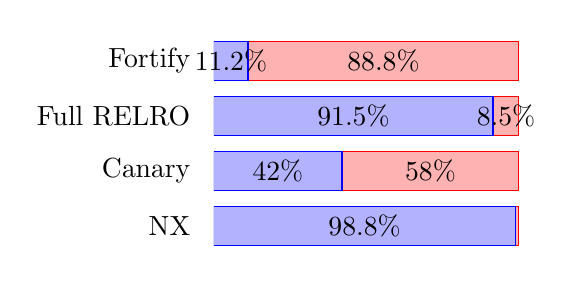
\begin{tikzpicture}
 \begin{axis}[testbar]
\addplot[draw=blue, fill=blue!30] coordinates{(98.8, 0) (42.0, 1) (91.5, 2) (11.2, 3)};\addplot[draw=red, fill=red!30] coordinates{(1.2, 0) (58.0, 1) (8.5, 2) (88.8, 3)};\end{axis}
 \end{tikzpicture}
